\documentclass{fefu}

\usepackage{graphicx}
\usepackage{float}
\usepackage{wrapfig}

\begin{document}
	\setschool{ШКОЛА ЕСТЕСТВЕННЫХ НАУК}
	\setdepartment{кафедра информатики, математического и компьютерного 
	моделирования}{А.Ю.Чеботарев}
	\setgroup{Б8403а}
	\title{о прохождении преддипломной практики\\направление подготовки 01.03.02 
	Прикладная математика и информатика\\профиль «Системное программирование»}
	\setdates{29}{апреля}{2019}{22}{июня}{2019}
	\setweeks{8}
	\setplace{кафедре информатики, \\математического и компьютерного \\моделирования}
	\author{Куцелабский Е.С.}
	\setsupervisor{Кленин А.С.}
	
	\makereporttitle
	\tableofcontents
	\newpage
	
	\begin{abstract}
		\par Текущая версия текстового редактора в open-source движке Citrus малоэффективна.
		Целью данной работы является разработка нового текстового редактора для 
		движка. В работе изложены особенности реализации и принятые решения.
		Выполнено сравнение производительности между предыдущей версией редактора и
		новой реализацией.
		\par \textbf{ОБНОВИТЬ объем кода, поменять таблицы на fefutable}
	\end{abstract}

	\section{Введение}
		\subsection{Глоссарий}
			\begin{itemize}
				\item Игровой движок --- базовое ПО игры, набор основных библиотек, на основе
				которых строится весь игровой проект
				\item Частота кадров --- количество сменяемых кадров в единицу времени
				\item Алгоритмическая сложность --- функция зависимости объема работы от 
				размера входных данных
				\item Soft wrap --- процесс разбиения файла на текстовые строки, при котором
				в случае, если строка не помещается в доступную ширину, часть слов будет
				перенесена на следующую строку
				\item Open-source --- ПО с исходным кодом, доступным для просмотра, изучения, 
				изменения
			\end{itemize}
		\subsection{Описание предметной области}
			\subsubsection{Студия Game Forest}
				\par Заказчиком данной работы выступает студия Game Forest. \cite{GFPortal} 
				Студия занимается созданием игр, и за время своего существования выпустила 
				более 40 проектов, суммарная аудитория которых -- более 100 млн человек. 
				Игровые проекты получали высокие оценки игроков, критиков и издателей, наиболее 
				успешной игрой, в данный момент, является Gummy Drop (количество скачиваний -- 
				более 50 млн)\cite{GummyDropPage}.
				\par Основой игровых проектов, в данный момент, является разработка студии -- 
				игровой движок Citrus. Он позволяет создавать приложения для нескольких
				платформ: Windows, MacOS, Android, iOS.
				\par Несмотря на существование крупных открытых игровых движков, таких как 
				Unity \cite{UnitySite} и Unreal Engine \cite{UnrealEngineSite}, 
				в Game Forest было принято решение использовать собственную разработку. К 
				такому же решению пришли многие крупные компании, например, Bethesda Game 
				Studios \cite{BethesdaEngine} и id Software \cite{idSoftwareEngine}.
				\par Крупные движки содержат инструменты для разработки игр всех жанров. 
				Создание и поддержка подобных инструментов даже на базовом уровне требует 
				огромных усилий, а учитывая тот факт, что подобные движки рассчитаны
				на массовую (часто непрофессиональную) аудиторию, комфорт и простота
				использования ставятся превыше производительности, что отрицательно сказывается
				на конечном продукте. Именно поэтому компании принимают решение о разработке
				собственных движков, создаваемых с учетом нужд компании. В подобных движках
				отсутствуют лишние компоненты, присущие массовым движкам, что позволяет
				сосредоточиться на улучшении действительно важных частей системы.
				\par Стоит отметить, что, в отличие от конкурентов, студия Game
				Forest распространяет свой движок под лицензией GPL-3.0, что позволяет
				использование, модификацию и распространение движка другими студиями и
				отдельными пользователями.
			\subsubsection{Игровой движок Citrus}
				\par Citrus состоит из нескольких взаимосвязанных модулей, каждый из которых
				реализует определенную функциональность (см. Рис. \ref{img:CitrusScheme})
				\cite{CitrusRepo}: 
				\begin{itemize}
					\item Yuzu --- библиотека, предоставляющая средства сериализации
					\item Kumquat --- генератор кода
					\item Lemon --- модуль компоновки сторонних библиотек
					\item Lime --- ядро движка
					\item Orange --- сборщик проектов, созданных при помощи движка
					\item Tangerine --- редактор сцен
				\end{itemize}
				\par Движок предоставляет возможность визуализации 2D и 3D графики, 
				оконных интерфейсов, поддерживает воспроизведение звуков, сборку проектов для 
				нескольких платформ, проигрывание и редактирование анимаций (в визуальном 
				редакторе). Компоненты активно дорабатываются, набор поддерживаемых функций, 
				при необходимости, дополняется.
				\par В модуле Lime, помимо прочего, содержатся части системы, ответственные за
				работу с текстом.
				\begin{figure}[h]
					\centering
					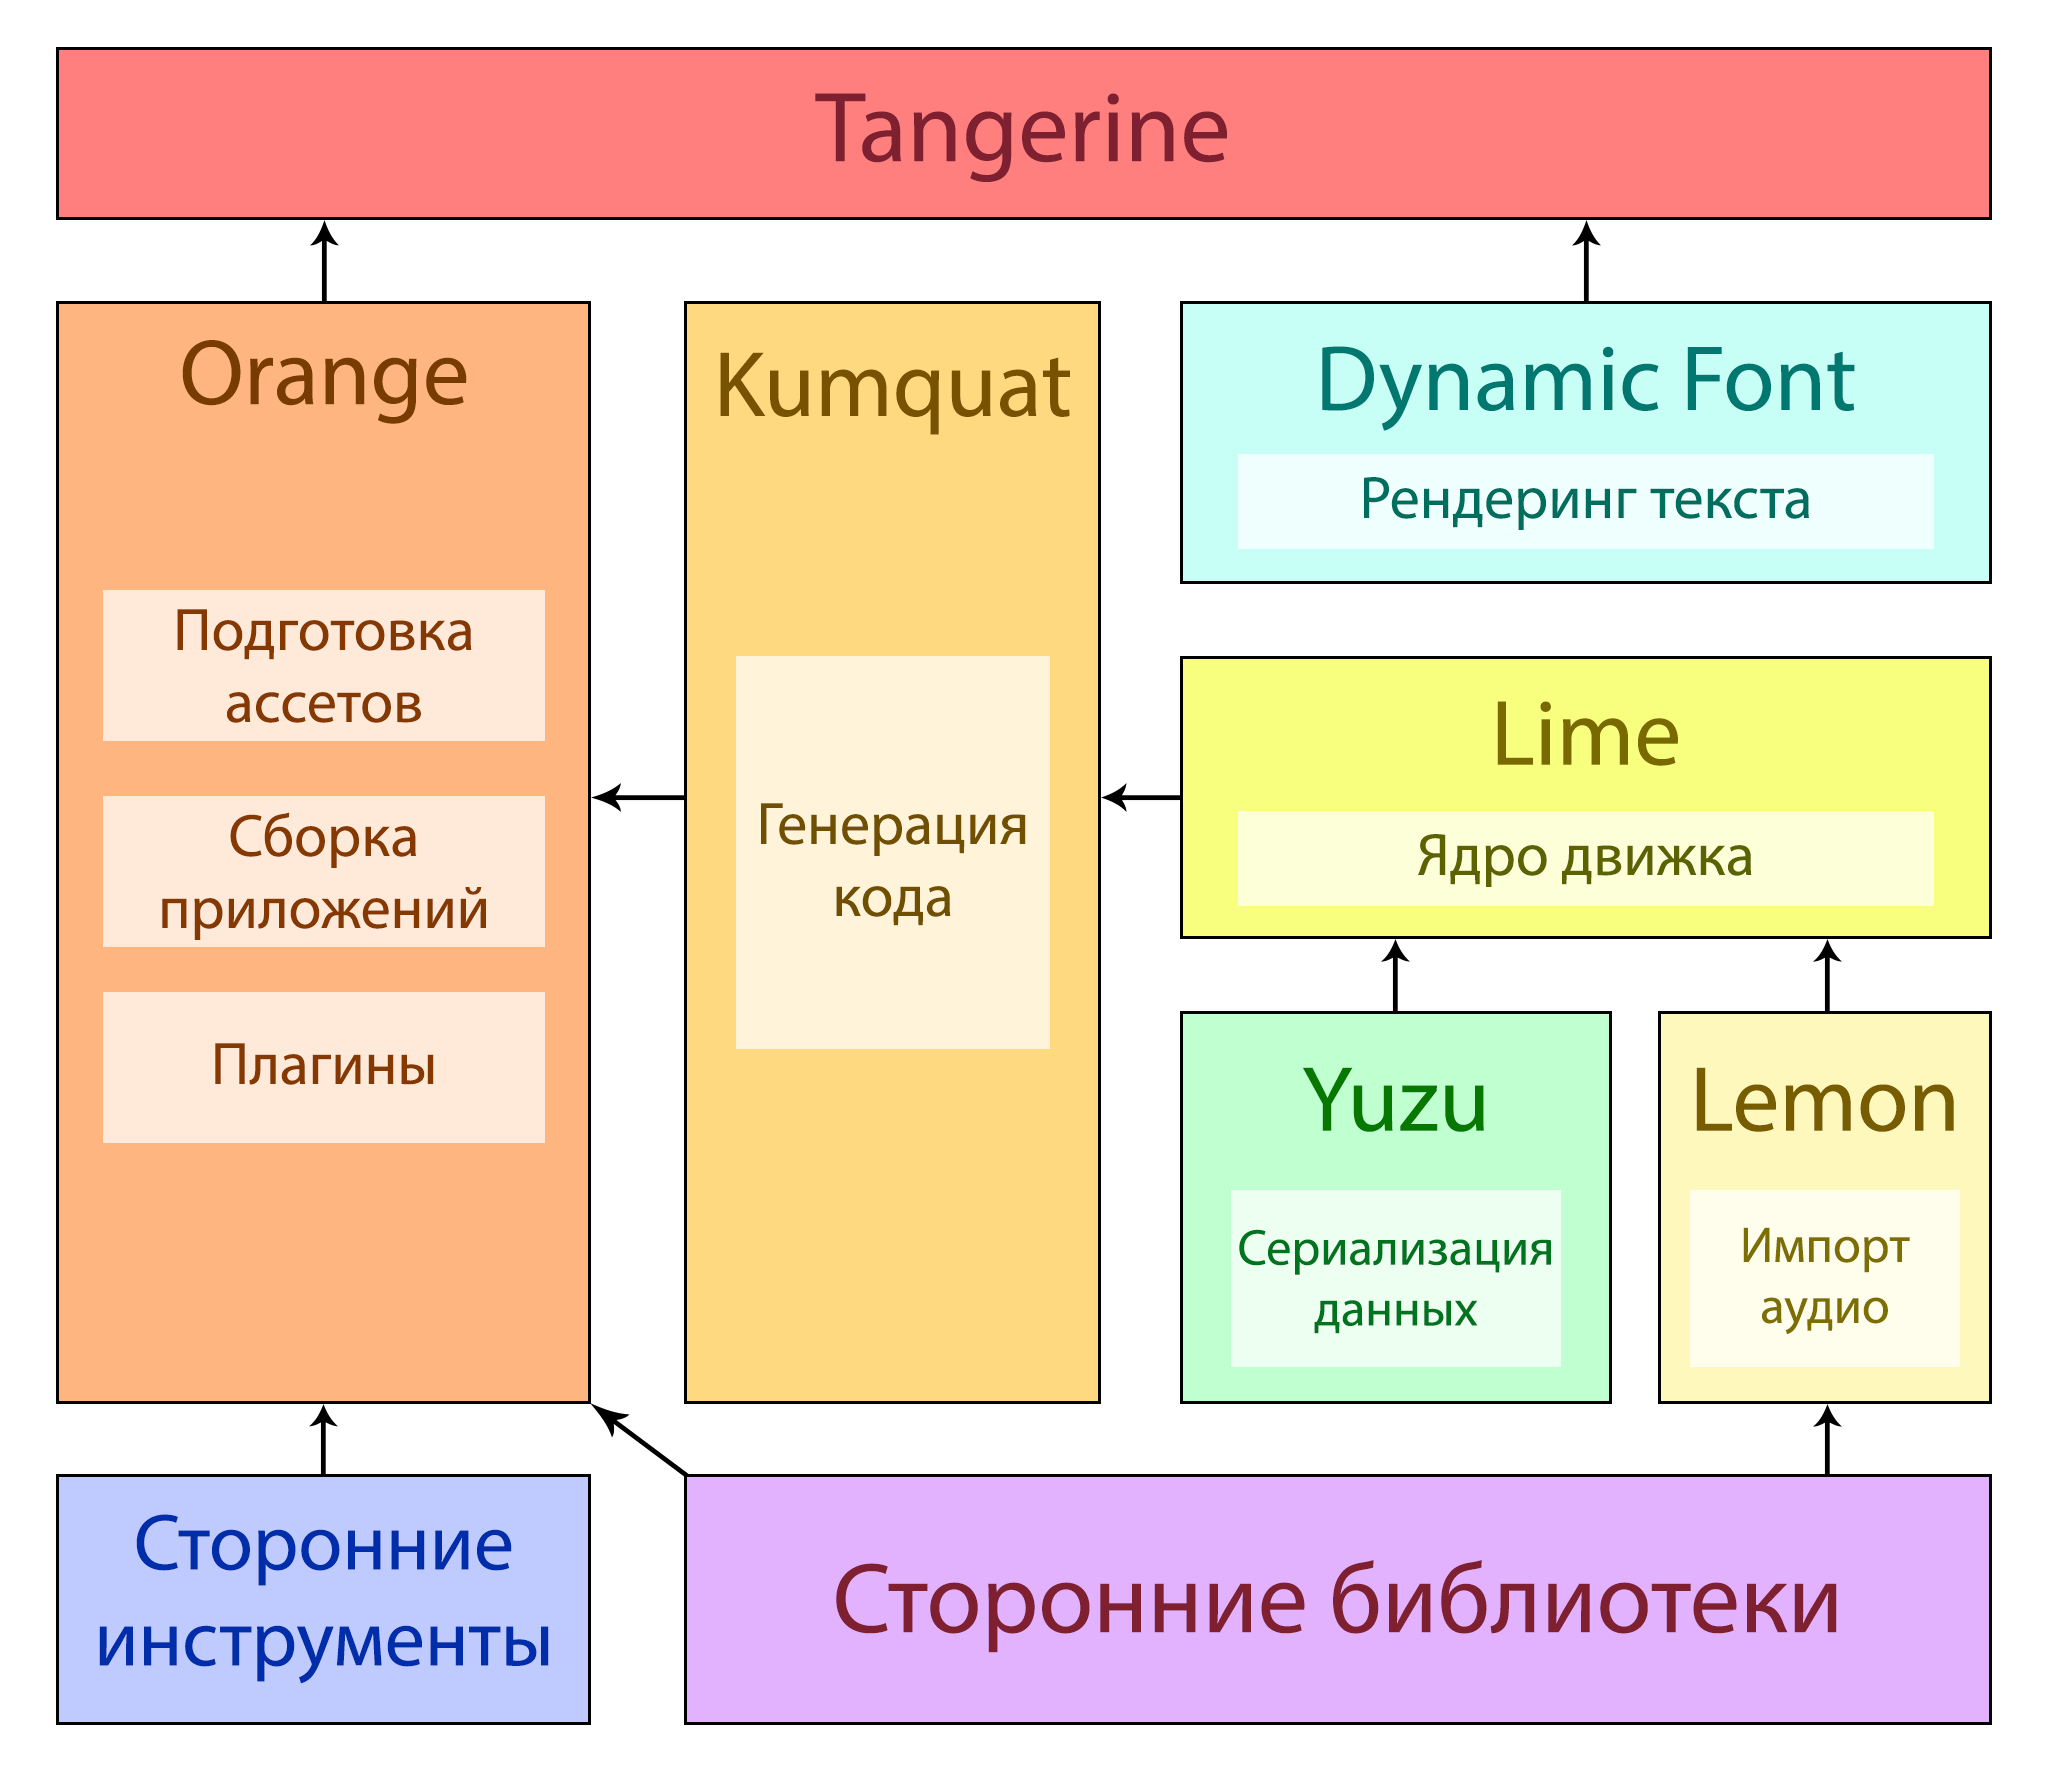
\includegraphics[width=1\linewidth]{images/CitrusScheme.png}
					\caption{Схема модулей движка Citrus}
					\label{img:CitrusScheme}
				\end{figure}
			\subsubsection{Текстовый редактор}
				\par Текстовый редактор это компьютерная программа (или её часть), 
				предназначенная для создания и изменения текстовых данных (в том числе 
				текстовых файлов). Часто редакторы предоставляют пользователям дополнительные 
				возможности, такие как: копирование и вставка, поиск и замена текста, 
				форматирование текста (переносы строк, выравнивание и пр.), 
				откат/восстановление изменений \cite{WhatIsATextEditor}. 
				\par Некоторые редакторы, помимо работы с обычным текстом, позволяют также и
				работу со стилизованным текстом (т.н. Rich Text) 
				\cite{DiffBetweenTextFormats}. Так как текстовый формат данных не предполагает
				хранения информации о стиле текста, в редакторах тексты обрамляются в различные
				языки разметки (например, HTML), либо используется внутреннее двоичное 
				представление.
				\par Для успешной работы текстового редактора необходимо, чтобы были
				реализованы три его основные компоненты: \cite{CraftOfTextEditing}
				\begin{enumerate}
					\item Обработка внутреннего представления текста --- текст необходимо
					эффективным образом хранить и изменять, наивный подход к этой части
					редактора приведёт к значительному (в случае работы с большими объемами
					данных -- к фатальному) падению производительности всего редактора.
					\item Отрисовка --- текст необходимо правильно отрисовать с учетом размеров
					окна и применённых стилей (шрифт, выравнивание, переносы слов).
					\item Обработка пользовательского ввода --- приём команд
					(вставка, удаление элемента, перевод курсора и~пр.) и передача их
					обработчику внутреннего представления.
				\end{enumerate}
			\subsubsection{Обработка текста в Citrus}
				\par Представление текстовых данных и работа с ними -- важная часть игрового
				движка, поскольку значительная часть важной игровой информации сообщается 
				пользователю в текстовом виде. 
				\par В Citrus есть классы, обеспечивающие обработку ввода и отрисовку текста 
				(см. Рис. \ref{diag:CitrusTextSystem}), 
				однако они реализованы неэффективно, что выражается в резком падении 
				производительности с увеличением длины текста. Это приводит к увеличению
				требований к процессору для поддержания высокой частоты кадров. При дальнейшем
				увеличении объема текста работа программ сильно замедляется, что критично для
				игровых проектов, и составляет значительные неудобства при работе со средствами
				визуального редактирования в движке. Также, несмотря на
				возможность корректно отображать многострочный текст, текущая система слабо
				приспособлена для его редактирования.
				\begin{figure}[h]
					\centering
					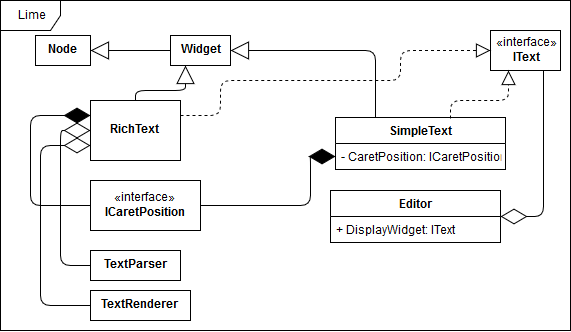
\includegraphics[width=1\linewidth]{diagrams/CitrusTextSystem.png}
					\caption{Диаграмма классов текстовой системы движка Citrus}
					\label{diag:CitrusTextSystem}
				\end{figure}
				\par В данный момент эти проблемы решаются обходным путём, т.е. число
				использований многострочного редактора сведено к минимуму, а появления больших
				объемов текста стараются, по возможности, не допускать. В игровых проектах
				число больших текстов невелико, а во время работы с визуальной частью движка
				неэффективность работы текстовой системы, хоть и замедляет работу, не является
				критическим препятствием.
				\par Для решения данных проблем можно переписать всю систему работы с текстом с
				нуля, а можно лишь оптимизировать малоэффективные части. Поскольку разработка 
				подобной системы связана со значительными трудностями, в то время как на уже
				существующую систему опираются многие игровые проекты, я решил лишь внести 
				необходимые изменения в существующую структуру работы.
				\par Первую часть системы -- обработку внутреннего представления текста -- 
				можно использовать как самостоятельную единицу в любых других проектах. Все 
				прочие части завязаны на существующую архитектуру движка Citrus и без него 
				неприменимы.
		\subsection{Неформальная постановка задачи}
			В рамках данной работы требуется выполнить следующие задачи:
			\begin{enumerate}
				\item Изучить имеющиеся подходы к реализации текстовых редакторов
				\item Создать редактор, обеспечивающий:
				\begin{itemize}
					\item Просмотр и редактирование обычного (не стилизованного) текста
					\item Поддержку работы с многострочными файлами
					\item Эффективную отрисовку больших объемов текста
					\item Поддержку стандартных пользовательских команд
				\end{itemize}
				\item Сравнить производительность новой и старой версий редактора
			\end{enumerate}
	\section{Обзор существующих методов решения}
		\subsection{Внутреннее представление текста}
			\par Для хранения и обработки текстовых данных используются различные подходы,
				хотя общее число зарекомендовавших себя относительно невелико.
				\cite{TextEditorDataStructures}.
			\par Для работы текстового редактора любая из структур должна поддерживать, как 
			минимум, следующие операции: вставку и удаление символов, получение элемента по его
			номеру, получение элемента по строке и столбцу, вставка/удаление в позиции курсора.
			\subsubsection{Массив символов}
				\par Наиболее очевидный способ хранения текста. Вся текстовая информация
				располагается в одном массиве. Это накладывает большие ограничения на скорость
				удаления и вставки \cite{StringsReference}. 
				\par Для удаления необходимо сдвинуть все элементы массива, начиная с позиции
				последнего удаляемого элемента, влево на число позиций, равное размеру
				удаляемой последовательности. Для вставки нужно сдвинуть все элементы, начиная
				с позиции вставки, вправо на число позиций, равное размеру удаляемой
				последовательности, а затем вставить последовательность в позицию вставки.
				\par Алгоритмическая сложность удаления и вставки -- $O(n)$. Учитывая 
				количество символов, зачастую присутствующее в тексте, это чудовищно плохой 
				показатель.
				\par Сложность получения элемента по номеру -- $O(1)$, поскольку достаточно
				применить адресную арифметику. В то же время, сложность получения элемента по
				строке и столбцу -- $O(n)$, потому что необходимо пробежаться по всем элементам
				массива, подсчитывая количество строк, до момента достижения необходимой
				позиции. Сложность вставки/удаления в позиции курсора -- $O(n)$.
				\par Несмотря на недостаточную эффективность, у подхода есть одно преимущество
				-- его очень легко реализовать. Однако для реализации чего-либо кроме
				простейшего однострочного поля ввода стоит предпочесть другие варианты.
			\subsubsection{Буферное окно (Gap buffer)}
				\par Текст хранится в массиве, однако часть строки не заполнена и служит для
				заполнения в случае необходимости вставки элемента. Так как в текстовых
				редакторах изменения, зачастую, происходят около одного места (позиция 
				курсора), то операции вставки и удаления можно выполнять очень быстро.
				Узким местом подхода является тот факт, что при интенсивных вставках элементов
				буфер может закончиться, в этом случае его необходимо будет расширить заново,
				выполнив операцию сдвига всех элементов вправо с определенной позиции на размер
				буфера. Перемещение буфера к позиции курсора так же требует времени, в худшем 
				случае (курсор переместили от начала текста к его концу) необходимо сдвинуть
				все элементы в массиве \cite{GapBufferArticle}.
				\par Утверждение об эффективности подхода опирается на предположение о том, что 
				стоимость перемещения курсора и расширения буфера амортизируется с помощью 
				прочих, дешевых операций, поскольку операции перемещения курсора и расширения 
				буфера довольно редки по сравнению с операциями вставки.
				\par Алгоритмическая сложность удаления и вставки, в худшем случае, $O(n)$. Для
				данного подхода затруднительно оценить среднестатистическую сложность.
				\par Сложность получения элемента по индексу, как и в случае с обычным 
				массивом, $O(1)$, адресная арифметика всё так же применима при условии, что
				текущий размер буфера всегда известен. Сложность получения элемента по строке и
				столбцу, по тем же причинам, что и у обычного массива, составляет $O(n)$.
				\par Данный подход легко реализуем и даёт значительный прирост
				производительности по сравнению с использованием обычного массива, однако он не
				рассчитан на работу с большими файлами, поскольку в них стоимость операций 
				перемещения курсора и расширения буфера чрезвычайно высоки.
				\par Сложность вставки в позицию курсора -- $O(1)$ (при условии, что 
				вставляемый текст не превосходит текущий размер буфера, иначе $O(n)$), 
				сложность удаления в позиции курсора -- всегда $O(1)$, поскольку удаления
				расширяют буфер без необходимости сдвигать элементы. Именно благодаря этому
				свойству этот метод часто используется в реализации текстовых редакторов.
				Считается, что стоимость редких операций расширения и перемещения буфера
				компенсируется быстрыми операциями вставки и удаления.
				\par Данный подход нашел применение во многих текстовых
				редакторах, в том числе в весьма известных (например, Emacs
				\cite{EmacsGapBuffer}).
				\par Пример работы. Исходное состояние:
				$$Lorem~ipsum~dolor~sit~[~~~~~~~~~~~~]~adipiscing.$$
				\par Пользователь добавляет текст:
				$$Lorem~ipsum~dolor~sit~amet,[~~]~adipiscing.$$
				\par Пользователь перемещает курсор
				$$Lorem~ipsum~dolor~sit~[~~]~amet,~adipiscing.$$
				\par Пользователь добавляет текст, полностью заполняющий буфер. Система
				расширяет буфер:
				$$Lorem~ipsum~dolor~sit~consectetur[~~~~~~~~~~]~amet,~adipiscing.$$
			\subsubsection{Связный список}
				\par Элементы (например, символы) хранятся в узлах односвязного списка. При 
				таком подходе операции вставки и удаления в позиции курсора выполняются очень 
				быстро, поскольку сводятся к манипуляциям с указателями. Проблемой в данном 
				случае становится операция получения элемента по некоторому индексу, поскольку 
				необходимо пройти по указателям от начала и до требуемого элемента, что в 
				худшем случае занимает $O(n)$ времени (для получения элемента по номерам строки
				и столбца сложность та же), причём эту операцию требуется выполнить и для 
				вставки или удаления элементов. Помимо прочего, на хранение большого числа 
				узлов требуется колоссальный объем памяти, поскольку в одном узле хранится лишь 
				по одному символу \cite{LinkedListReference}.
				\par Преимуществом этого подхода является тот факт, что в узлах, помимо
				информации о символе, можно хранить и прочую информацию, например, информацию
				о стиле текста.
			\subsubsection{Набор строк}
				\par Предыдущие варианты реализации текстовых редакторов не ориентированы на
				применение в многострочных редакторах. Использование набора строк --
				естественное решение этой проблемы. Текст представляется в виде набора
				массивов, каждый из которых хранит только по одной строке текста. Стоит
				отметить, что вместо обычных массивов можно использовать описанные выше
				подходы для увеличения эффективности. Использование набора строк позволяет
				оптимизировать отрисовку. Зная номера строк, в данный момент помещающихся в 
				активное окно, можно быстро к ним обратиться и отрисовать только строго
				необходимый объем текста. 
				\par Этот подход раскрывается при использовании в многострочных редакторах,
				поскольку позволяет за $O(1)$ обращаться к элементам по номерам строки и
				столбца. При вставке в позицию курсора, поскольку номер строки заранее 
				известен, сложность составит $O(k)$, где $k$ -- количество символов в строке.
				В случае вставки по номеру символа в тексте необходимо сначала пробежаться по
				всем строкам, подсчитав число символов в них, чтобы найти строку для вставки.
				Сложность подобной операции составит $O(s + k)$, где $s$ -- количество строк,
				$k$ -- количество символов в строке.
			\subsubsection{Верёвка (Rope)}
				\par Структура данных для хранения информации о строках, представляющая собой
				двоичное дерево, в листах которых хранятся текстовые строки, а в узлах 
				информация о размере (в символах) поддеревьев (см. Рис. \ref{img:RopeExample})
				\cite{RopeArticle}.
				\begin{figure}[h]
					\centering
					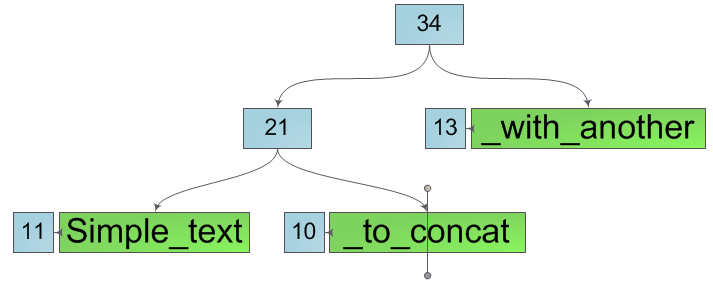
\includegraphics[width=1\linewidth]{images/RopeExample.png}
					\caption{Пример применения структуры Rope}
					\label{img:RopeExample}
				\end{figure}
				\par В изначальном представлении балансировка не предполагается, однако без неё
				стоимость операций значительно увеличивается, поэтому при описании сложности
				операций будем предполагать, что был применён некоторый алгоритм балансировки.
				\par Сложность операций вставки и удаления -- $O(\log{m})$, где $m$ - высота
				дерева. Для проведения операции необходимо спуститься от корня к нужному листу,
				по пути обновляя информацию о размере поддеревьев. После этого разделение
				(в случае необходимости) или удаление листа дерева и вставка нового элемента
				выполняются за $O(1)$.
				\par Операция доступа к элементу по его номеру также выполняется за 
				$O(\log{m})$, в то время как операция доступа к элементу по номерам строки и
				столбца, без дополнительных оптимизаций, выполняется за $O(n)$, потому-что 
				необходимо пробежаться по всему тексту.
				\par К сожалению, наличие курсора никак не ускоряет вставку элементов в его
				позиции, поскольку обход дерева в любом случае должен быть совершен для
				обновления размеров в узлах. Сложность этой операции остается прежней -- 
				$O(\log{m})$.
			\subsubsection{Таблица кусочков (Piece Table) и расширяющееся дерево (Splay tree)}
				\par Таблица кусочков - эффективная структура данных, используемая во многих 
				современных текстовых редакторах \cite{PieceTableArticle}. Используется 
				несколько потоков (файлов) -- исходный и добавочный. Исходный поток 
				используется только для чтения. В добавочный данные добавляются и читаются из 
				него, но не удаляются. Вместо хранения самих символов, в структуре хранится 
				информация о текстовых фрагментах, а именно: позиция начала фрагмента в потоке 
				(файле), его длина, исходный ли это поток или добавочный. При добавлении новых 
				символов они записываются в добавочный поток, а в таблицу заносится новый 
				фрагмент. При вставке текста, в случае если позиция нового фрагмента содержится 
				внутри существующего, возможно разбиение фрагментов на две части, тогда в левой 
				части фрагмента остаётся информация о части текста, лежащей до нового 
				фрагмента, а в правой -- после (см. Рис. \ref{img:PieceTableExample}). Во время 
				удаления от фрагментов "отрезаются" части, либо весь фрагмент удаляется 
				целиком.
				\begin{figure}[h]
					\centering
					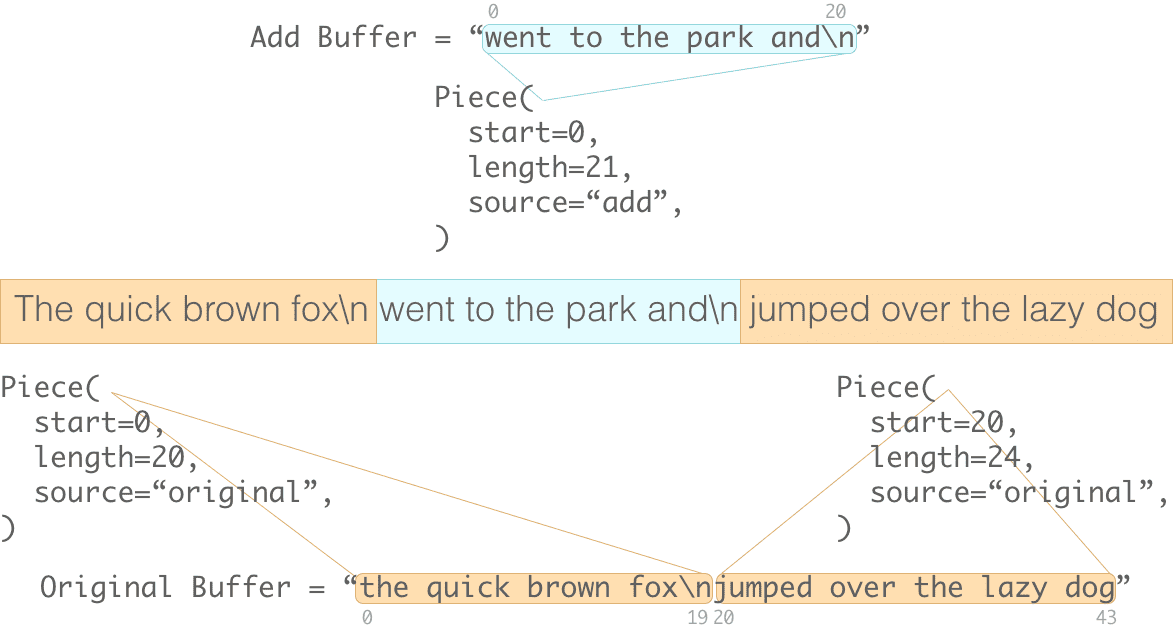
\includegraphics[width=1\linewidth]{images/PieceTableExample.png}
					\caption{Пример применения структуры Piece Table}
					\label{img:PieceTableExample}
				\end{figure}
				\par Таблица кусочков это лишь структура данных для хранения информации о
				тексте, настоящую эффективность данному подходу придаёт способ хранения
				кусочков. Одним из наиболее эффективных способов является использование 
				расширяющегося дерева (Splay Tree). Это сбалансированное бинарное дерево 
				поиска, в котором элементы, к которым в последний раз было произведено
				обращение, перемещаются в корень. Это свойство особенно эффективно при
				использовании в текстовых редакторах, поскольку в них большая часть изменений
				производится около одного места -- позиции курсора \cite{SplayTreeArticle}.
				Автором работы для связки было выбрано название "Piece Tree". Данный подход
				используется в нескольких современных текстовых редакторах, например, в 
				Atom \cite{TextEditorsHabr}.
				\par При использовании расширяющегося дерева сложность вставки и удаления
				составляет $O(\log{m})$, где $m$ -- высота дерева. Операция получения
				элемента так же выполняется за $O(\log{m})$.
				\par Операция получения элемента по номерам строки и столбца в случае наивной
				реализации имеет сложность $O(n)$, где $n$ -- число символов в тексте, однако
				зачастую применяются различные техники для оптимизации этой операции.
				\par Все вышеперечисленные сложности описаны для худшего случая, в случае
				работы с текстом в позиции курсора операции будут выполнены значительно 
				быстрее, поскольку все необходимые элементы будут находиться близко к корню
				дерева, благодаря чему для достижения нужной позиции не потребуется совершать
				полный пробег по дереву. Сложность операций в этом случае -- $O(1)$.
				\par Дополнительным преимуществом подхода является тот факт, что он
				использует значительно меньше памяти, чем прочие, поскольку вместо хранения,
				непосредственно, символов, хранится лишь набор ссылок на части текста.
			\subsubsection{Сравнение}
				\par{Для наглядности построим сравнительную таблицу (см. Табл. 
				\ref{table:MethodComplexity})}
				\begin{table}[H]
					\centering
					\begin{tabular}{|p{4cm}|*{4}{p{3cm}|}}
						\hline 
						\textbf{Подход} & \textbf{Вставка и удаление} & 
						\textbf{Обращение по номеру} & \textbf{Обращение по 
						координатам} & \textbf{Вставка в позиции курсора}\\
						\hline
						Массив & $O(n)$ & $O(1)$ & $O(n)$ & $O(n)$ \\
						\hline
						Буферное окно & $O(n)$ & $O(1)$ & $O(n)$ & $O(1)$ \\
						\hline
						Связный список & $O(n)$ & $O(n)$ & $O(n)$ & $O(1)$ \\
						\hline
						Набор строк & $O(s + k)$ & $O(1)$ & $O(1)$ &  $O(k)$ \\
						\hline
						Rope & $O(\log{m})$ & $O(\log{m})$ & $O(n)$ & $O(\log{m})$ \\
						\hline
						Piece Tree & $O(\log{m})$ & $O(\log{m})$ & $O(n)$ & $O(1)$ \\
						\hline
					\end{tabular}
					\caption{Сравнение алгоритмических сложностей подходов}
					\label{table:MethodComplexity}
				\end{table}
				\par Здесь:
				\begin{itemize}
					\item $s$ --- кол-во строк 
					\item $k$ --- кол-во символов в строке
					\item $m$ --- высота дерева
				\end{itemize}
				\par К сожалению, для многих подходов трудно вывести алгоритмическую сложность
				в среднем случае, многое зависит от ряда оговорок и условий работы. Тем не
				менее, учитывая описанные выше особенности подходов, можно с уверенностью
				утверждать, что таблица кусочков -- это наиболее эффективный способ организации
				внутреннего представления текста.
	\section{Требования к окружению}
		\subsection{Требования к аппаратному обеспечению}
			\par Поскольку текстовый редактор является частью движка Citrus и не существует 
			без него, то ниже приведены общие требования для запуска движка и игровых проектов,
			сделанных на его основе.
			\begin{itemize}
				\item GPU с поддержкой OpenGL ES 2.0 либо Vulkan либо Molten VK
				\item CPU с частотой 1 ГГц или выше
				\item 512 Мб RAM или больше
			\end{itemize}
		\subsection{Требования к программному обеспечению}
			\par Поскольку текстовый редактор является частью движка Citrus и не существует 
			без него, то ниже приведены общие требования для запуска движка и игровых проектов,
			сделанных на его основе.
			\begin{itemize}
				\item ОС Windows 8.1 или выше; macOS 10.13 или выше; дистрибутивы 
				Linux, поддерживающие среду Mono; Android 5 или выше; iOS 10.3.3 или выше
				\item .NET Framework версии 4.7.1 или выше
			\end{itemize}
	\section{Архитектура системы}
		\par Систему можно поделить на три модуля:
		\begin{enumerate}
			\item Модуль обработки внутреннего представления текста --- отвечает за хранение
			текста и эффективное выполнение базовых операций (вставка, удаление, доступ).
			\item Модуль отрисовки --- обеспечивает корректную и эффективную отрисовку текста
			с учетом размеров виджета.
			\item Модуль обработки пользовательского ввода --- отвечает за получение
			пользовательских команд и отправку их в обработчик внутреннего представления.
		\end{enumerate}
	\section{Спецификация данных}
		\subsection{Описание формата или структуры данных}
			\par Данная реализация текстового редактора не предполагает поддержку
			стилизованного текста, однако подобная функциональность заложена в архитектуру.
			Для указания информации о стиле будут использоваться тэги, подобные тем, что
			используются в HTML.
	\section{Функциональные требования}
		\par Модуль обработки внутреннего представления текста должен уметь:
		\begin{itemize}
			\item Хранить текст
			\item Вставлять текстовую строку в позицию курсора (\textit{Здесь и далее под текстовой позицией 
			понимается номер элемента, перед которым будет применена операция, под
			позицией курсора понимаются номера строки и столбца, на которые в данный момент
			ссылается курсор}).
			\item Удалять текстовый фрагмент определённого размера, 
			начиная с позиции курсора.
			\item Выделять текстовый фрагмент определённого размера.
			\item Удалять предыдущий/следующий за курсором символ.
			\item Перемещать курсор на позицию предыдущего/следующего
			за курсором элемента.
			\item Перемещать курсор в начало / конец текущей строки
			\item Перемещать курсор на строку вверх/вниз.
			\item Перемещать курсор на определенную текстовую позицию.
			\item Расширять/сужать выделение на предыдущий/следующий за курсором элемент.
			\item Копировать, вырезать и, впоследствии, вставлять выделенный текстовый 
			фрагмент.
			\item Отменять предыдущую выполненную операцию.
			\item Повторно выполнять предыдущую отмененную операцию.
			\item Получать вест текущий текст в формате текстовой 
			строки.
		\end{itemize}
		\par Модуль отрисовки должен:
		\begin{itemize}
			\item Выполнять отрисовку текста в заданном окне в рамках прямоугольной области, 
			параметры которой задаются программистом, с учетом параметров шрифта.
			\item Обеспечивать перенос слов на следующую строку, в случае, если
			текущая строка по горизонтали не помещается в видимую область, при условии, что 
			данный режим переноса активирован (soft wrap).
			\item Отрисовывать только видимую часть текста, отбрасывая строки, в данный момент
			не попадающие в видимую область
			\item Обеспечивать возможность вертикальной и/или горизонтальной прокрутки 
			текста
			\item Выполнять отрисовку курсора в его текущей позиции
		\end{itemize}
		\par Модуль обработки пользовательского ввода должен:
		\begin{itemize}
			\item Обрабатывать ввод текстовых данных с клавиатуры
			\item Перемещать курсор в определенном направлении соответственно нажатой 
			клавише "Вверх", "Вниз", "Влево" или "Вправо"
			\item По клику мышью/касанию экрана в области обработки текста перемещать курсор
			в позицию клика/касания
			\item Выделять текст в диапазоне, заданном кликом/касанием с протягиванием по
			области обработки текста
			\item По нажатию клавиши "Enter" вставлять в текст перевод строки
			\item По нажатию на клавиши "Home" и "End" переводить курсор в начало/конец строки
			соответственно
			\item Обрабатывать нажатия на комбинации "Shift + Влево", "Shift + Вправо", 
			"Shift + Вниз", "Shift + Вверх", "Shift + Home", "Shift + End", переводя курсор
			в соответствующую позицию с применением выделения
			\item По нажатию на клавиши "Delete" и "Backspace" удалять следующий/предыдущий
			(за позицией курсора) символ
			\item Обрабатывать нажатия на комбинации "Ctrl + Влево", "Ctrl + Вправо", 
			"Ctrl + Backspace", "Ctrl + Delete", применяя результаты соответствующих команд без
			модификатора "Ctrl" к словам (вместо отдельных символов)
			\item Обрабатывать нажатия на комбинации "Ctrl + Shift + Влево", 
			"Ctrl + Shift + Вправо", перемещая курсор на слово влево/вправо с применением
			выделения
			\item Обрабатывать вызов контекстного меню и выбор в нём действия (способ вызова
			меню зависит от платформы: для ПК способом вызова меню является клик правой
			кнопкой мыши по области редактора, для мобильных устройств - долгое касание в 
			области обработки текста)
		\end{itemize}
	\section{Требования к интерфейсу}
		\par Текстовый редактор предназначен для оконных интерфейсов. Интерфейс представляет
		собой прямоугольник в заданной области окна, внутри которого рисуется текст и курсор. Окно редактора может обладать 
		вертикальным скроллбаром, горизонтальным или никаким. Для взаимодействия с редактором
		используются клавиши клавиатуры, 
		аппаратной или электронной, действия контекстного меню, клики мыши/касания экрана.
		\par Текст может рисоваться с применением разных настроек шрифта, с использованием soft
		wrap или без него.
	\section{Прочие требования}
		\subsection{Требования к производительности}
			Вся цепочка операций (от обработки изменений текста до 
			отрисовки) должна выполняться не более чем за 30 миллисекунд (для отрисовки 30 
			кадров в секунду) для многострочных файлов порядка нескольких мегабайт на экранах
			разрешением порядка 1024x768. Требования указаны для устройств, имеющих
			производительность сравнимую с iPhone 5 (или лучшую).
	\section{Проект}
		\subsection{Средства реализации}
			Все части системы были реализованы на языке C\# 7.0, 
			версия .NET Framework 4.7.1, поскольку это стандарт для компании Game Forest.
		\subsection{Структуры данных}
			\subsubsection{PieceTreeNode}
				\par Узел расширяющегося дерева, хранит информацию о 
				текстовых фрагментах (см. Таблица \ref{table:PieceTreeNode}).
				\begin{table}[h]
					\centering
					\begin{tabular}{|l|l|p{10cm}|}
						\hline
						\textbf{Имя поля} & \textbf{Тип данных} & \textbf{Описание} \\
						\hline
						Left & PieceTreeNode & Ссылка на левого потомка\\
						\hline
						Right & PieceTreeNode & Ссылка на правого потомка \\
						\hline
						Parent & PieceTreeNode & Ссылка на родителя \\
						\hline
						Owner & PieceTree & Ссылка на дерево, содержащее данный узел \\
						\hline
						Position & Целое число & Позиция, с которой фрагмент начинается в 
						итоговом тексте \\
						\hline
						Length & Целое число & Длина текстового фрагмента \\
						\hline
						IsOrigin & Логический тип & Истинно, если фрагмент является частью 
						исходного потока \\
						\hline
						FilePosition & Целое число & Позиция начала фрагмента в потоке \\
						\hline
					\end{tabular}
					\caption{Структура PieceTreeNode}
					\label{table:PieceTreeNode}
				\end{table}
			\subsubsection{PieceTree}
				\par Расширяющееся дерево, узлами которого являются
				PieceTreeNode. В нём выполняются все операции, необходимые для поиска,
				вставки, удаления элементов, а так же операции undo и redo (см. Таблица 
				\ref{table:PieceTree}). Сбалансированность дерева достигается благодаря системе
				поворотов, осуществляемых во время перемещения элемента в корень дерева. 
				Используется три вида поворотов:
				\begin{itemize}
					\item Zig --- Если $p$ -- корень дерева с ребенком $x$, то выполняется один
					поворот вокруг ребра $(x, p)$ (см. Рис. \ref{img:zig})
					\item Zig-zig --- Если $p$ -- не корень дерева, $x$ -- его ребенок, а $x$ и 
					$p$ оба левые или правые дети, то делаем поворот ребра $(p, g)$, где $g$ 
					отец $p$, а потом делаем поворот ребра $(x, p)$ (см. Рис. \ref{img:zigzig})
					\item Zig-zag --- Если $p$ -- не корень дерева, $x$ -- его левый 
					ребенок, а $p$ правый ребенок своего отца (или наоборот), то делаем
					поворот вокруг ребра $(x, p)$, а затем поворот нового ребра $(x, g)$, где 
					$g$ -- бывший родитель $p$ (см. Рис. \ref{img:zigzag})
				\end{itemize}
				\begin{figure}[H]
					\centering
					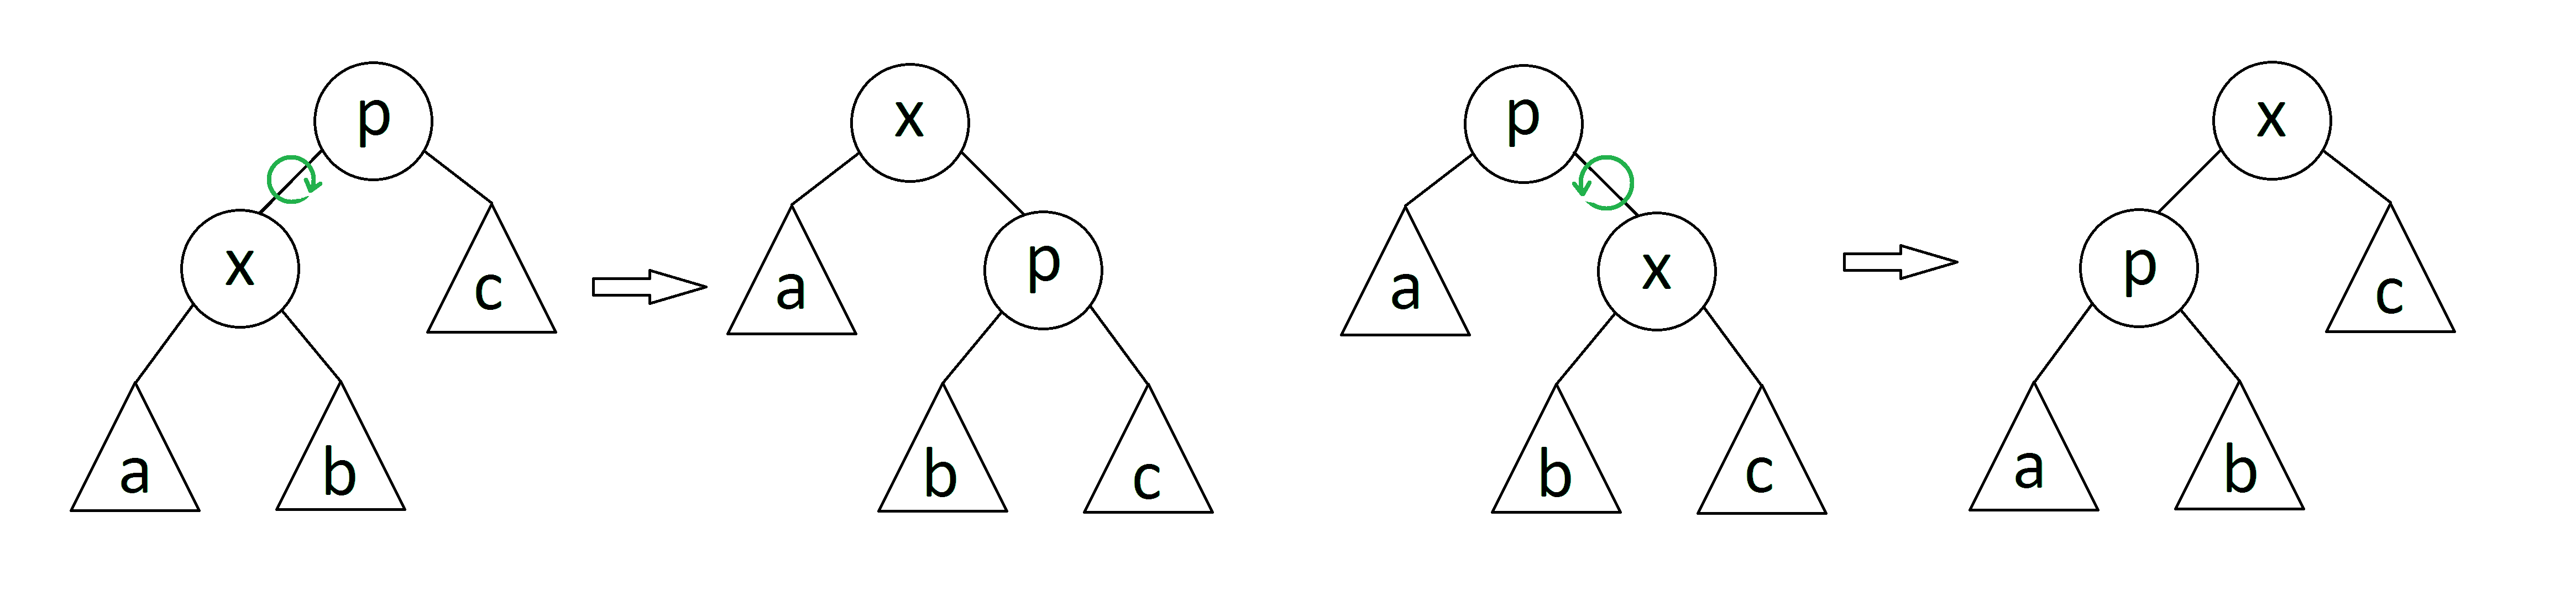
\includegraphics[width=0.8\linewidth]{images/zig.png}
					\caption{Поворот Zig}
					\label{img:zig}
				\end{figure}
				\begin{figure}[H]
					\centering
					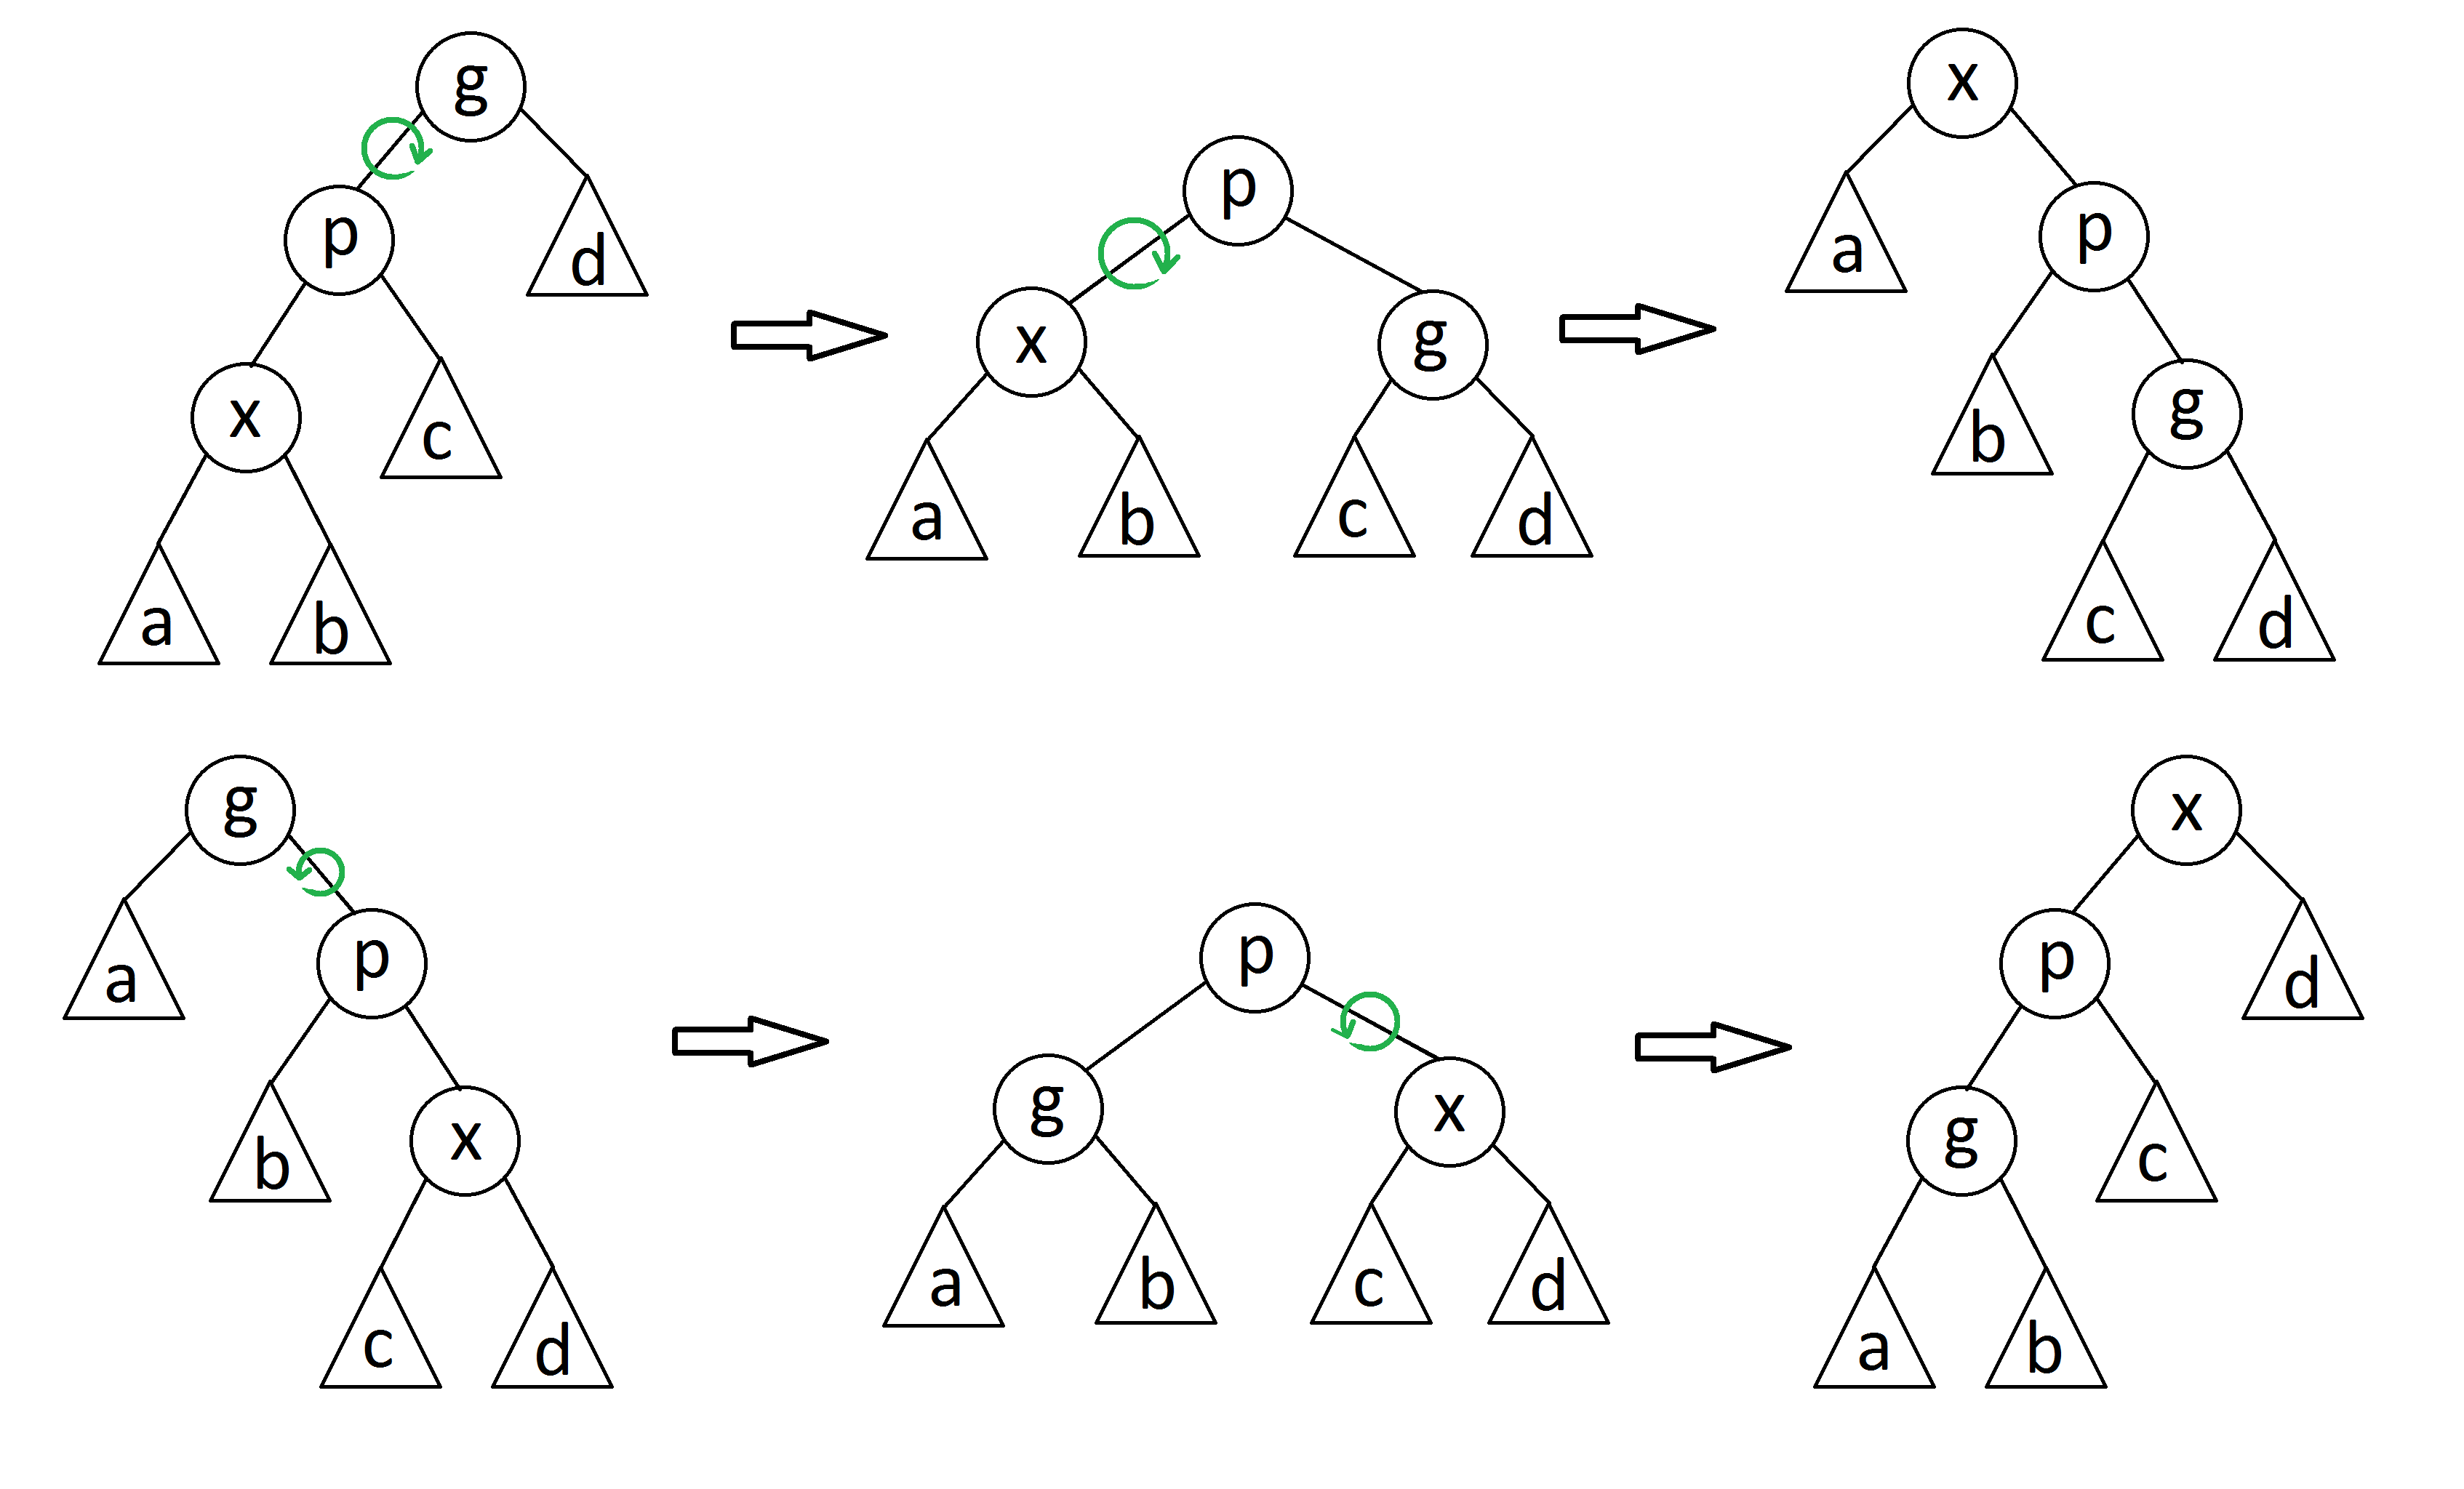
\includegraphics[width=0.8\linewidth]{images/zigzig.png}
					\caption{Поворот Zig-zig}
					\label{img:zigzig}
				\end{figure}
				\begin{figure}[H]
					\centering
					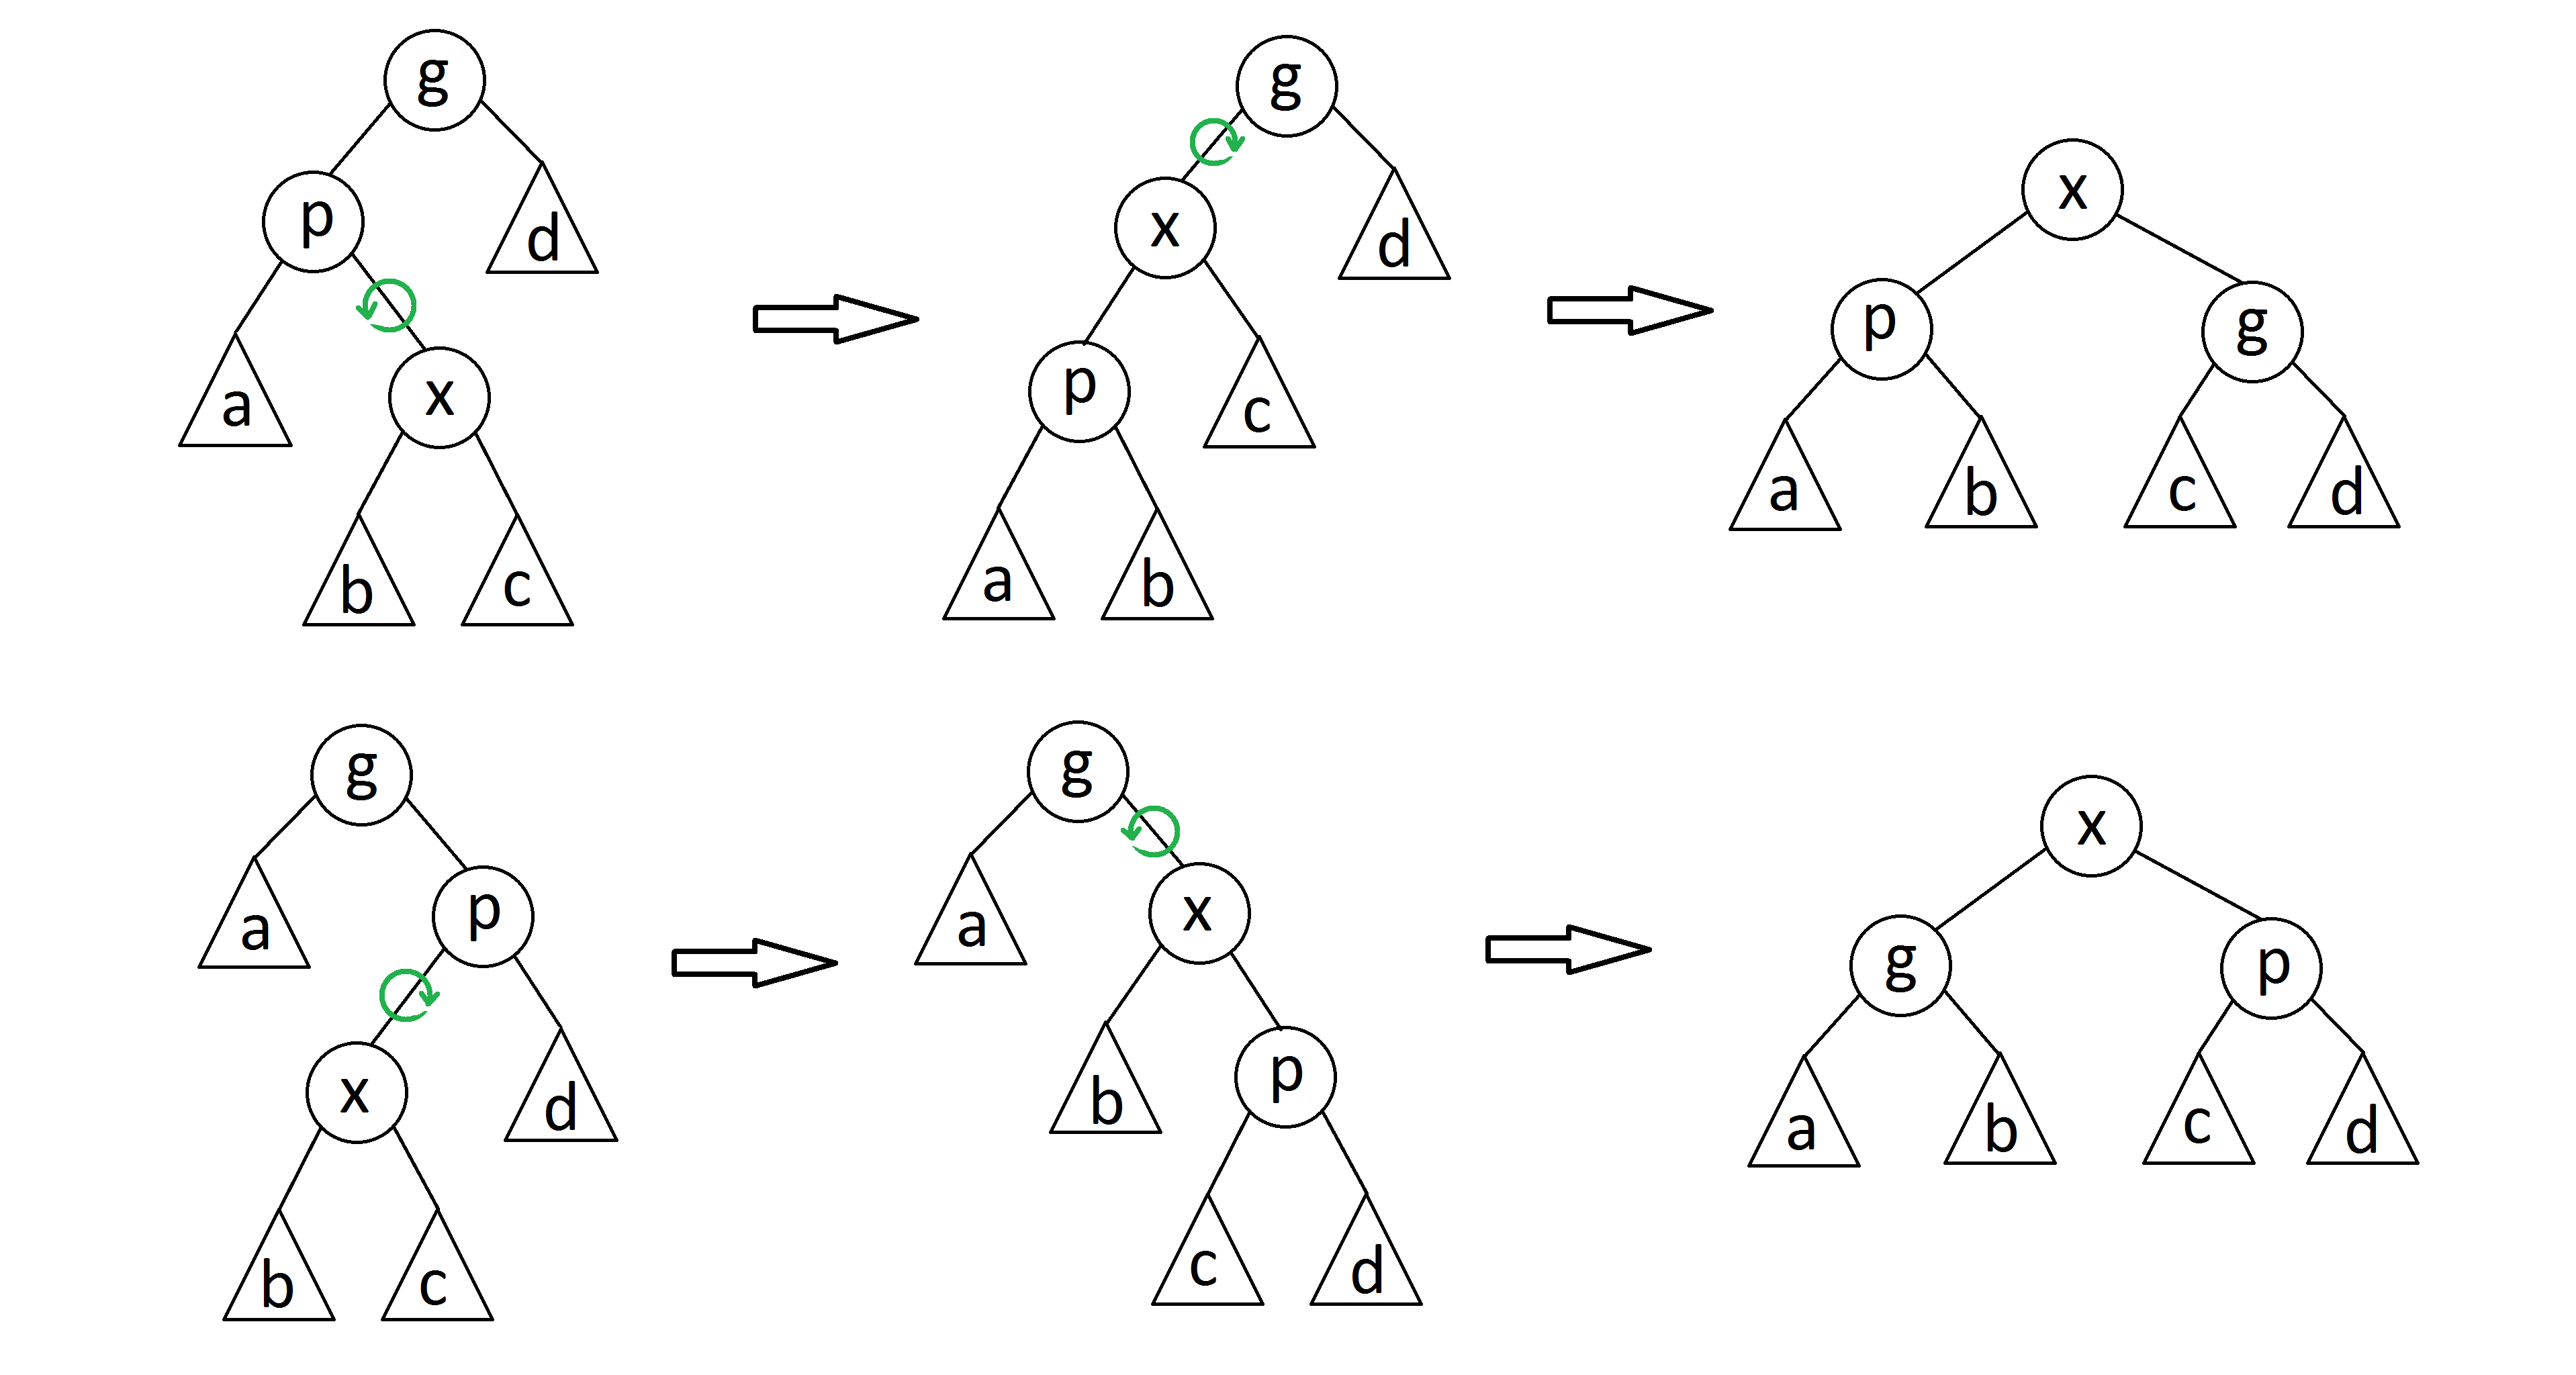
\includegraphics[width=0.8\linewidth]{images/zigzag.png}
					\caption{Поворот Zig-zag}
					\label{img:zigzag}
				\end{figure}
				\par Существует лемма \cite{SplayTreeArticle}, доказывающая, что 
				амортизационная сложность операции не превосходит $O(\log{n})$, где $n$ -- 
				число узлов.
				\begin{table}[H]
					\centering
					\begin{tabular}{|l|l|p{10cm}|}
						\hline
						\textbf{Имя поля} & \textbf{Тип данных} & \textbf{Описание} \\
						\hline
						Root & PieceTreeNode & Ссылка на корень дерева \\
						\hline
						OriginStream & Поток данных & Ссылка на исходный поток данных \\
						\hline
						AddStream & Поток данных & Ссылка на добавочный поток данных \\
						\hline
						undoStack & UndoStack & Ссылка на структуру, хранящую стек операций \\
						\hline
					\end{tabular}
					\caption{Структура PieceTree}
					\label{table:PieceTree}
				\end{table}
			\subsubsection{Word}
				\par Структура для хранения информации об отдельном слове (см. Таблица 
				\ref{table:Word}).
				\begin{table}[h]
					\centering
					\begin{tabular}{|l|l|p{9cm}|}
						\hline
						\textbf{Имя поля} & \textbf{Тип данных} & \textbf{Описание} \\
						\hline
						TextIndex & Целое число & Позиция в массиве текстов \\
						\hline
						Start & Целое число & Номер первого символа слова в тексте \\
						\hline
						Length & Целое число & Длина слова \\
						\hline
						ForceLineBreak & Логический тип & Истинно, если перед словом стоял
						символ переноса строки\\
						\hline 
						X & Вещественное число & Позиция в пикселях по горизонтали \\
						\hline 
						Width & Вещественное число & Ширина в пикселях \\
						\hline
						LineBreak & Логический тип & Истинно, если слово необходимо перенести
						на следующую строку из-за soft-wrap \\
						\hline
						IsNbsp & Логический тип & Истинно, если слово содержит неразрывный
						пробел\\
						\hline
					\end{tabular}
					\caption{Структура Word}
					\label{table:Word}
				\end{table}
			\subsubsection{Line}
				\par Структура для хранения информации о строках текста (см. Таблица 
				\ref{table:Line}).
				\begin{table}[H]
					\centering
					\begin{tabular}{|l|l|p{9cm}|}
						\hline
						\textbf{Имя поля} & \textbf{Тип данных} & \textbf{Описание} \\
						\hline
						Position & Целое число & Номер в тексте первого символа первого слова 
						\\
						\hline
						Length  & Целое число & Длина строки в символах \\
						\hline
						StartWordIndex & Целое число & Индекс первого слова в массиве слов \\
						\hline
						WordCount & Целое число & Количество слов в строке \\
						\hline
						Width & Вещественное число & Ширина строки в пикселях \\
						\hline
						Height & Вещественное число & Высота строки в пикселях \\
						\hline
						Offset & Вещественное число & Суммарная высота предыдущих строк \\
						\hline
					\end{tabular}
					\caption{Структура Line}
					\label{table:Line}
				\end{table}
			\subsubsection{Command}
				\par Вспомогательная структура данных для операций undo/redo. Хранит в себе
				копию части дерева определенного размера, в зависимости от типа хранимой
				команды и операции выполняет вставку копии в основное дерево или удаление
				части основного дерева (см. Таблица \ref{table:Command}).
				\begin{table}[h]
					\centering
					\begin{tabular}{|l|l|p{9cm}|}
						\hline
						\textbf{Имя поля} & \textbf{Тип данных} & \textbf{Описание} \\
						\hline
						CommandType & Перечисляемый тип & Тип команды, может быть "Insert" или 
						"Delete" \\
						\hline
						Node & PieceTreeNode & Корневой узел хранимой копии дерева \\
						\hline
					\end{tabular}
					\caption{Структура Command}
					\label{table:Command}
				\end{table}
		\subsection{Модули и алгоритмы}
			\subsubsection{Обработка внутреннего представления текста}
				\par Данный модуль состоит из следующих классов (см. Рис. 
				\ref{diag:SubEditorScheme}):
				\begin{itemize}
					\item CaretPosition --- описывает положение курсора и 
					обрабатывает его перемещение.
					\item Selection --- хранит информацию о текущем выделении, обрабатывает его
					изменения
					\item UndoStack --- хранит стек обработанных операций, по запросу PieceTree 
					сообщает необходимые данные
					\item SubEditor --- связующее звено между модулями. Принимает команды на 
					редактирование текста и перемещение курсора, перенаправляет их
					соответствующим модулям
				\end{itemize}
				\begin{figure}[h]
					\centering
					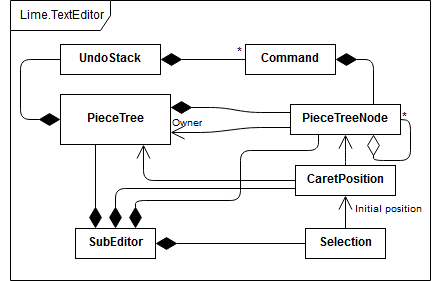
\includegraphics[width=1\linewidth]{diagrams/SubEditorScheme.png}
					\caption{Диаграмма классов модуля обработки внутреннего 
					представления текста}
					\label{diag:SubEditorScheme}
				\end{figure}
			\subsubsection{Модуль отрисовки}
				\par Данный модуль состоит из следующих классов (см. Рис. 
				\ref{diag:RendererScheme}):
				\begin{itemize}
					\item TextParser --- выделяет из текста фрагменты (отдельные слова, 
					переносы строк, пробелы)
					\item TextRenderer --- получает набор фрагментов от TextParser, для каждого
					фрагмента определяет его позицию в тексте, учитывая параметры шрифта и 
					размеры окна, при необходимости применяет soft wrap, затем передаёт
					полученные данные в общий рендерер движка, который выполняет
					непосредственную отрисовку
					\item CommonText --- содержит в себе SubEditor, TextParser и TextRenderer,
					обеспечивает обмен данными между ними, помимо этого содержит информацию о
					параметрах шрифта. Стоит отметить, что в случаях, когда необходимо лишь 
					отобразить текст без возможности редактирования, достаточно возможностей
					этого класса
				\end{itemize}
				\begin{figure}[h]
					\centering
					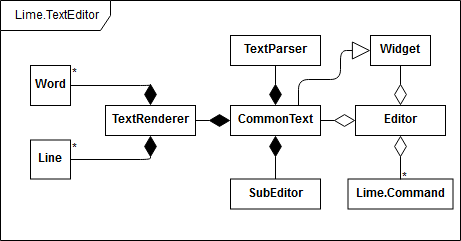
\includegraphics[width=1\linewidth]{diagrams/EditorScheme.png}
					\caption{Диаграмма классов модулей отрисовки и пользовательского
					ввода}
					\label{diag:RendererScheme}
				\end{figure}
			\subsubsection{Модуль обработки пользовательского ввода}
				\par Вся функциональность данного модуля содержится в классе Editor. Он
				обрабатывает пользовательский ввод, перенаправляя команды в SubEditor,
				находящийся внутри CommonText, который является полем в Editor (см. Рис. 
				\ref{diag:RendererScheme}).
			\subsubsection{Виджет прокрутки}
				\par Поскольку существующий модуль прокрутки не позволял оптимизировать
				отрисовку, были созданы следующие классы (см. Рис. \ref{diag:ScrollView}):
				\begin{itemize}
					\item ScrollView --- класс, использующий CommonText для отрисовки текста,
					обеспечивающий передачу ему информации о текущей видимой его части, а так
					реализующий возможность прокрутки
					\item ScrollViewWithSlider --- потомок класса ScrollView, добавляющий в 
					него слайдер, который можно тянуть пальцем или мышью, и реализующий его
					поведение
					\item ThemedScrollView --- потомок класса ScrollViewWithSlider,
					реализующий настройку визуальной составляющей виджета и слайдера
					\item ThemedTextView --- потомок класса ThemedTextView, реализующий 
					операцию "Добавить текст"
				\end{itemize}
				\begin{figure}[H]
					\centering
					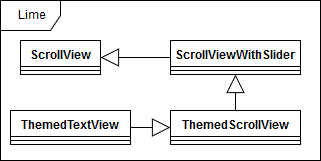
\includegraphics[width=0.7\linewidth]{diagrams/ScrollView.png}
					\caption{Диаграмма классов виджетов прокрутки}
					\label{diag:ScrollView}
				\end{figure}
		\subsection{Проблемы и решения}
			\par В ходе разработки пришлось столкнуться со следующими проблемами:
			\begin{itemize}
				\item Выбор структуры данных вызвал затруднения, поскольку необходимо было
				соблюсти баланс между эффективностью и сложностью разработки. Тем не менее,
				было принято решение использовать наиболее эффективный подход, несмотря на 
				потенциальные сложности при реализации.
				\item Необходимо было выбрать способ реализации операций undo и redo.
				Существует два подхода: инверсия операции и хранение информации о состоянии.
				Автором работы было принято решение об использовании инверсии операций. Для
				этого, в момент выполнения операции вставки, в стек сохраняется
				вставляемый фрагмент. Во время выполнения операции удаления в стек сохраняется
				удаляемая часть дерева. Для этого выполняется почленное клонирование входящих
				в дерево узлов, при необходимости узлы обрезаются до необходимого размера. 
				После этого полученное поддерево кладется в стек. При необходимости отменить
				предыдущую операцию, полученное поддерево берётся из стека и, в случае отмены
				удаления, выполняется операция вставки этого поддерева, а в случае отмены
				вставки выполняется удаления части дерева с границами, соответствующими
				границам сохраненного поддерева.
				\item Текущая архитектура не позволяла проводить тестирование скорости 
				прокрутки, поскольку она всегда рисовала виджет целиком и показывала лишь 
				видимую его часть, что в корне противоречит идее оптимизации. Было принято
				решение написать новый класс на основе старого, позволяющий отрисовывать только
				видимую часть текста и не тратить ресурсы на остальную.
				\item Самой большой проблемой является необходимость при редактировании текста
				эффективно пересчитывать координаты символов в нескольких координатных
				системах (позиция в тексте, строка и столбец, строка и столбец с учетом soft 
				wrap, пиксели). Затруднения вызывает тот факт, что информация для разных
				координатных систем хранится в разных структурах данных. Для решения проблемы
				был написан ряд методов-обработчиков, синхронизирующих данные между 
				структурами.
			\end{itemize}
		\subsection{Стандарт кодирования}
			Использован стандарт кодирования, принятый в Game Forest \cite{CodingConventions}.
		\subsection{Проект интерфейса}
			\par Автору работы не ставилась задача разработки конкретного вида интерфейса, за
			исключением архитектурных особенностей (отрисовка в ограниченном прямоугольнике).
			Тем не менее, в целях тестирования, были разработаны классы, поддерживающие 
			прокрутку нового текста.
			\begin{figure}[H]
				\centering
				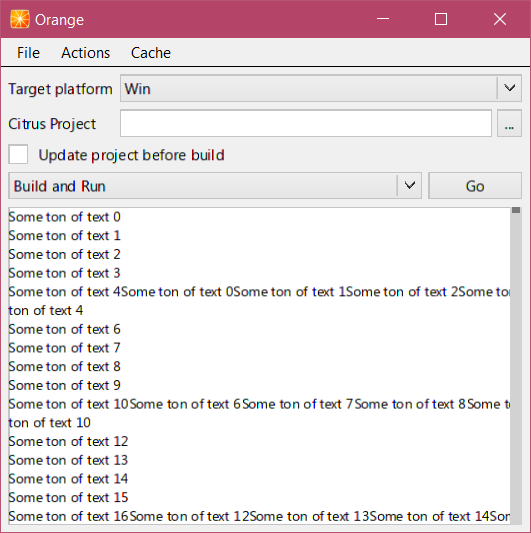
\includegraphics[width=0.5\linewidth]{images/ScrollViewInt.png}
				\caption{Интерфейс Citrus с встроенным ThemedTextView}
			\end{figure}
			\begin{figure}[H]
				\centering
				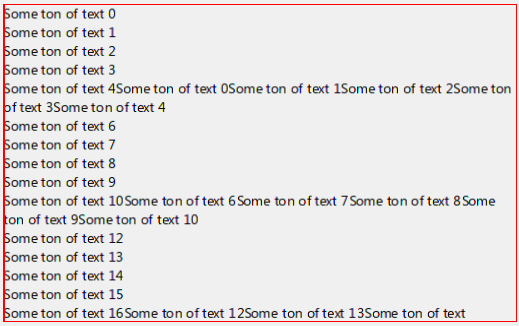
\includegraphics[width=0.5\linewidth]{images/CommonTextInt.png}
				\caption{Виджет CommonText. Включен режим подсветки 
				границ виджета}
			\end{figure}
			\begin{figure}[H]
				\centering
				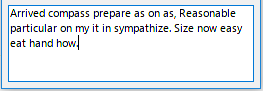
\includegraphics[width=0.5\linewidth]{images/EditBox.png}
				\caption{Виджет Editor}
			\end{figure}
			\begin{figure}[H]
				\centering
				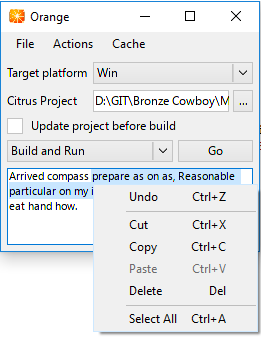
\includegraphics[width=0.5\linewidth]{images/EditorContextMenu.png}
				\caption{Интерфейс Citrus со встроенным Editor, открыто контекстное меню}
			\end{figure}
			\begin{figure}[H]
				\centering
				
\includegraphics[width=1\linewidth]{images/DecoratedBubble.png}
				\caption{Декорированный виджет CommonText}
			\end{figure}
	\section{Реализация и тестирование}
		\par Объем кода: 5132 строки, ~149 кб.
		\par Число коммитов: 58
		\par Количество автотестов: 63. Тестами покрывался модуль обработки внутреннего 
		представления текста, уровень покрытия -- 90\%.
		\par Репозиторий: https://github.com/mrojkov/Citrus
		\subsection{Вычислительный эксперимент}
			\par Было проведено сравнение скорости отрисовки в новой и старой версиях 
			редактора при вызове операции перерисовки при изменении размера. Было выяснено, что 
			новая версия редактора в разы превосходит по скорости предыдущую, причём её 
			производительность не деградирует при увеличении количества строк в тексте (см. 
			Рис. \ref{img:RenderComparisonBig} и Рис. \ref{img:RenderComparisonSmall}).
			\begin{figure}[h]
				\centering
				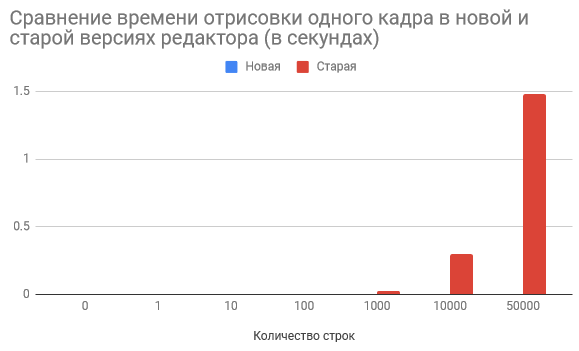
\includegraphics[width=0.8\linewidth]{images/RenderComparisonBig.png}
				\caption{Сравнение времени отрисовки одного кадра в новой и старой версиях 
				редактора (в секундах), максимальное число строк - 50000}
				\label{img:RenderComparisonBig}
			\end{figure}
			\begin{figure}[H]
				\centering
				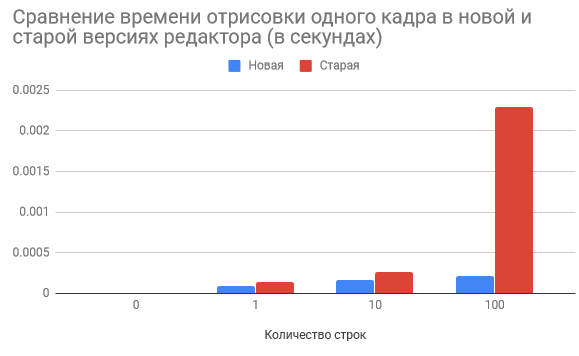
\includegraphics[width=0.8\linewidth]{images/RenderComparisonSmall.png}
				\caption{Сравнение времени отрисовки одного кадра в новой и старой версиях 
				редактора (в секундах), максимальное число строк - 100}
				\label{img:RenderComparisonSmall}
			\end{figure}
			\par Для операции вставки было проведено тестирование с замерами времени 
			выполнения:
			Операция последовательной вставки 30000 строк текста длиной 50 символов в конец
			текста в старой версии редактора занимает, в среднем 6.8 секунд. В новой 
			версии -- 4.3 секунды. При этом в старой версии текста, помимо прочего, после 
			каждой вставки пересчитывается новая позиция курсора.
	\section*{Заключение}
		\par Таким образом, в процессе выпускной квалификационной работы:
		\begin{itemize}
			\item Были исследованы подходы к реализации текстовых редакторов
			\item Был реализован текстовый редактор для open-source движка Citrus
			\item Было проведено сравнение производительности новой и старой версии текстовых
			редакторов
		\end{itemize}
		\par Были углублены знания в области:
		\begin{itemize}
			\item Языка программирования C\#
			\item Проектирования систем
			\item Работы с системами контроля версий
			\item Внутренних процессов компании Game Forest
		\end{itemize}
		\par Новый текстовый редактор поддерживает работу с многострочными файлами и работает
		значительно быстрее, чем предыдущий. В данный момент он находится в процессе опытной
		эксплуатации.
		\par В рамках дальнейшего развития можно реализовать поддержку стилизованного текста,
		а так же переосмыслить архитектуру модуля отрисовки для упрощения кода.
	\newpage
	\bibliographystyle{ugost2008ls}
	\bibliography{references}	
\end{document}